%%%%%%%%%%%%%%%%%%%%%%%%%%%%%%%%%%%%%%%%%%%%%%%%%%%%%%%%%%%%%%%%%%%%%%
% LaTeX Template: Two Column Colour Article
%
% Source: http://www.howtotex.com/
% Feel free to distribute this template, but please keep the
% referal to howtotex.com.
% Date: Feb 2011
% 
%%%%%%%%%%%%%%%%%%%%%%%%%%%%%%%%%%%%%%%%%%%%%%%%%%%%%%%%%%%%%%%%%%%%%%
% How to use writeLaTeX: 
%
% You edit the source code here on the left, and the preview on the
% right shows you the result within a few seconds.
%
% Bookmark this page and share the URL with your co-authors. They can
% edit at the same time!
%
% You can upload figures, bibliographies, custom classes and
% styles using the files menu.
%
% If you're new to LaTeX, the wikibook is a great place to start:
% http://en.wikibooks.org/wiki/LaTeX
%
%%%%%%%%%%%%%%%%%%%%%%%%%%%%%%%%%%%%%%%%%%%%%%%%%%%%%%%%%%%%%%%%%%%%%%

%%% Preamble
\documentclass[	DIV=calc,%
							paper=a4,%
							fontsize=11pt,%
							twocolumn]{scrartcl}	 					% KOMA-article class

\usepackage{lipsum}													% Package to create dummy text
\usepackage[utf8]{inputenc}
\usepackage[english]{babel}										% English language/hyphenation
\usepackage[protrusion=true,expansion=true]{microtype}				% Better typography
\usepackage{amsmath,amsfonts,amsthm}					% Math packages
\usepackage[pdftex]{graphicx}									% Enable pdflatex
\usepackage[svgnames]{xcolor}									% Enabling colors by their 'svgnames'
\usepackage[hang, small,labelfont=bf,up,textfont=it,up]{caption}	% Custom captions under/above floats
\usepackage{epstopdf}												% Converts .eps to .pdf
\usepackage{subfig}													% Subfigures
\usepackage{booktabs}												% Nicer tables
\usepackage{fix-cm}													% Custom fontsizes


\usepackage[bibnewpage]{apacite}
\usepackage[authoryear,round,longnamesfirst]{natbib} % bibliography fancy style


\usepackage{array}
\newcolumntype{L}[1]{>{\raggedright\let\newline\\\arraybackslash\hspace{0pt}}m{#1}}
\newcolumntype{C}[1]{>{\centering\let\newline\\\arraybackslash\hspace{0pt}}m{#1}}
\newcolumntype{R}[1]{>{\raggedleft\let\newline\\\arraybackslash\hspace{0pt}}m{#1}}


%%% Custom sectioning (sectsty package)
\usepackage{sectsty}													% Custom sectioning (see below)
\allsectionsfont{%															% Change font of al section commands
	\usefont{OT1}{phv}{b}{n}%										% bch-b-n: CharterBT-Bold font
	}

\sectionfont{%																% Change font of \section command
	\usefont{OT1}{phv}{b}{n}%										% bch-b-n: CharterBT-Bold font
	}




%%% Headers and footers
\usepackage{fancyhdr}												% Needed to define custom headers/footers
	\pagestyle{fancy}														% Enabling the custom headers/footers
\usepackage{lastpage}	


%Colores propios de el formato del informe
\definecolor{CiceBlue}{HTML}{1E3696}
\definecolor{CiceBlue2}{HTML}{6B92BC}
\definecolor{CiceBlue3}{HTML}{22487A}
\definecolor{CiceGray}{HTML}{585858}
\definecolor{CiceGray2}{HTML}{CCCCCC}

% Header (empty)
\lhead{}
\chead{}
\rhead{}
% Footer (you may change this to your own needs)
\lfoot{\footnotesize \texttt{siata.gov.co} \textbullet ~Initial version}
\cfoot{}
\rfoot{\footnotesize page \thepage\ of \pageref{LastPage}}	% "Page 1 of 2"
\renewcommand{\headrulewidth}{0.0pt}
\renewcommand{\footrulewidth}{0.4pt}



%%% Creating an initial of the very first character of the content
\usepackage{lettrine}
\newcommand{\initial}[1]{%
     \lettrine[lines=3,lhang=0.3,nindent=0em]{
     				\color{CiceBlue2}
     				{\textsf{#1}}}{}}



%%% Title, author and date metadata
\usepackage{titling}															% For custom titles

% \newcommand{\HorRule}{\color{DarkGoldenrod}%			% Creating a horizontal rule
% 									  	\rule{\linewidth}{1pt}%
% 										}
                                       
\newcommand{\HorRule}{\color{CiceGray}%			% Creating a horizontal rule
									  	\rule{\linewidth}{1pt}%
										}

\pretitle{\vspace{-30pt} \begin{flushleft} \HorRule 
				\fontsize{30}{40} \usefont{OT1}{phv}{b}{n} \color{CiceBlue3} \selectfont 
				}
% \title{Differences of stability indexes between days with absence of precipitation or days with presence of precipitation}					% Title of your article goes here
\title{Assessment of the variability of the thermodynamic structure of the atmosphere in the Aburrá Valley, Colombia. Part I: Influence on precipitation }
\posttitle{\par\end{flushleft}\vskip 0.5em}

\preauthor{\begin{flushleft}
					\large \lineskip 0.5em \usefont{OT1}{phv}{b}{sl} \color{CiceBlue3}}
\author{Carlos Cuervo, Carlos Hoyos, }											% Author name goes here
\postauthor{\footnotesize \usefont{OT1}{phv}{m}{sl} \color{Black} 
					 National University of Colombia 								% Institution of author
					\par\end{flushleft}\HorRule}


\date{}																				% No date 



%%% Begin document
\begin{document}
\maketitle
\thispagestyle{fancy} 			% Enabling the custom headers/footers for the first page 
% The first character should be within \initial{}
\initial{H}\textbf{ere is some sample of the thermodynamical difference of some stability indexes between days with absence of precipitation  or days with presence precipitation events.}

Precipitation is one of the most outstanding, dynamic and intermitent components of the hydrological cycle, and therefore of the climatic system. Water vapor, being one of the factors conditioning precipitation, plays a crucial role in different atmospheric processes. Water vapor varies in a wide range of temporal and spatial scales, from the local scale associated with microclimatic variability, to global scales associated with long-term climate change. The distribution of water vapor is related to cloud distribution, precipitation and atmospheric storms due to the large amount of latent heat released in the water’s phase change, which is also an important source of energy for air movement in the atmosphere. Besides, the distribution of water affects the vertical stability of the atmosphere, the structure and evolution of atmospheric storms, because these processes have great sensitivity to water vapor and temperature profiles, while also having implications in regional and global water and energy cycles. This research evaluates the variability of water vapor over the Aburrá Valley and its role on different thermodynamic processes of the troposphere at the start of precipitation events, mainly in events of convective origin. Different strategies were used, using remote and direct monitoring of the variables associated with thermodynamic processes in the atmosphere such as satellite sources like NASA’s AIRS (Atmospheric Infrared Sounder) products microwave radiometers (MWR ; \textit{MicroWave Radiometer}), 120 radiosoundings; finally applying modeling strategies to these processes using SIATA operational numerical modeling scheme, which is based on the WRF (Weather Research Forecast) model. With these different strategies water vapor and temperature profiles were obtained. The behavior of the thermodynamic vertical structure of the atmosphere was quantified using stability indexes, which evaluates the effectiveness of nowcasting of precipitation events over the Aburrá Valley. It also shows some of the stability conditions, and in general the thermodynamic conditions that favors the dispersion of pollutants. In these processes, the importance of having permanent measurements of the thermodynamic profiles of the troposphere was evidenced, mainly in the levels which are closer to the surface. where a better understanding of the thermodynamic phenomena associated with precipitation events and knowledge of the proper distribution of water vapor is needed not only during the beginning of the events but also during its extension and development with its drastic implications to air quality in the valley, mainly in terms of the extension of the atmospheric boundary layer.

\section{Introduction}
The precipitation is one of the most important components of the hydrological cycle, thus the climate system \citep{davies2011global}. The spatial an temporal variability of the precipitation as also this activation depends of dynamic, thermodynamic factors, local and remote forcings modulates the occurrence and also the magnitude, intensity and type of precipitation. One necessary condition for the precipitation formation is the phase change of the water vapor, this play a crucial role in diverse atmospheric processes, and is one of the principals constituents gases of the atmosphere, even though it constitutes only 0 to 4\% of the total volume of the atmosphere, it is the gas that contributes most efficiently to the greenhouse effect. The water vapor distribution is closely related with cloud distribution, precipitation and his intensification due to the large amount of latent heat liberated in the water phase change, that is an important source of energy to the air movement in the atmosphere.


To quantify the changes in the water vapor profiles of the atmosphere with absence and presence of precipitation events in the Figure \ref{fig:VaporDifference} shows the difference of the diurnal cycles of water vapor in the days with absence of precipitation and the days with presence of precipitation events in the Aburr\'a Valley, in this is clear to see the importance of the increment of water vapor density in the afternoons at the low an middle troposphere. The afternoons are the  hours of the mos common intense precipitation events over the Aburr\'a Valley. \textbf{ (poner ciclo diurno de lluvias de EPM???)}

\begin{figure}[h!]
\centering
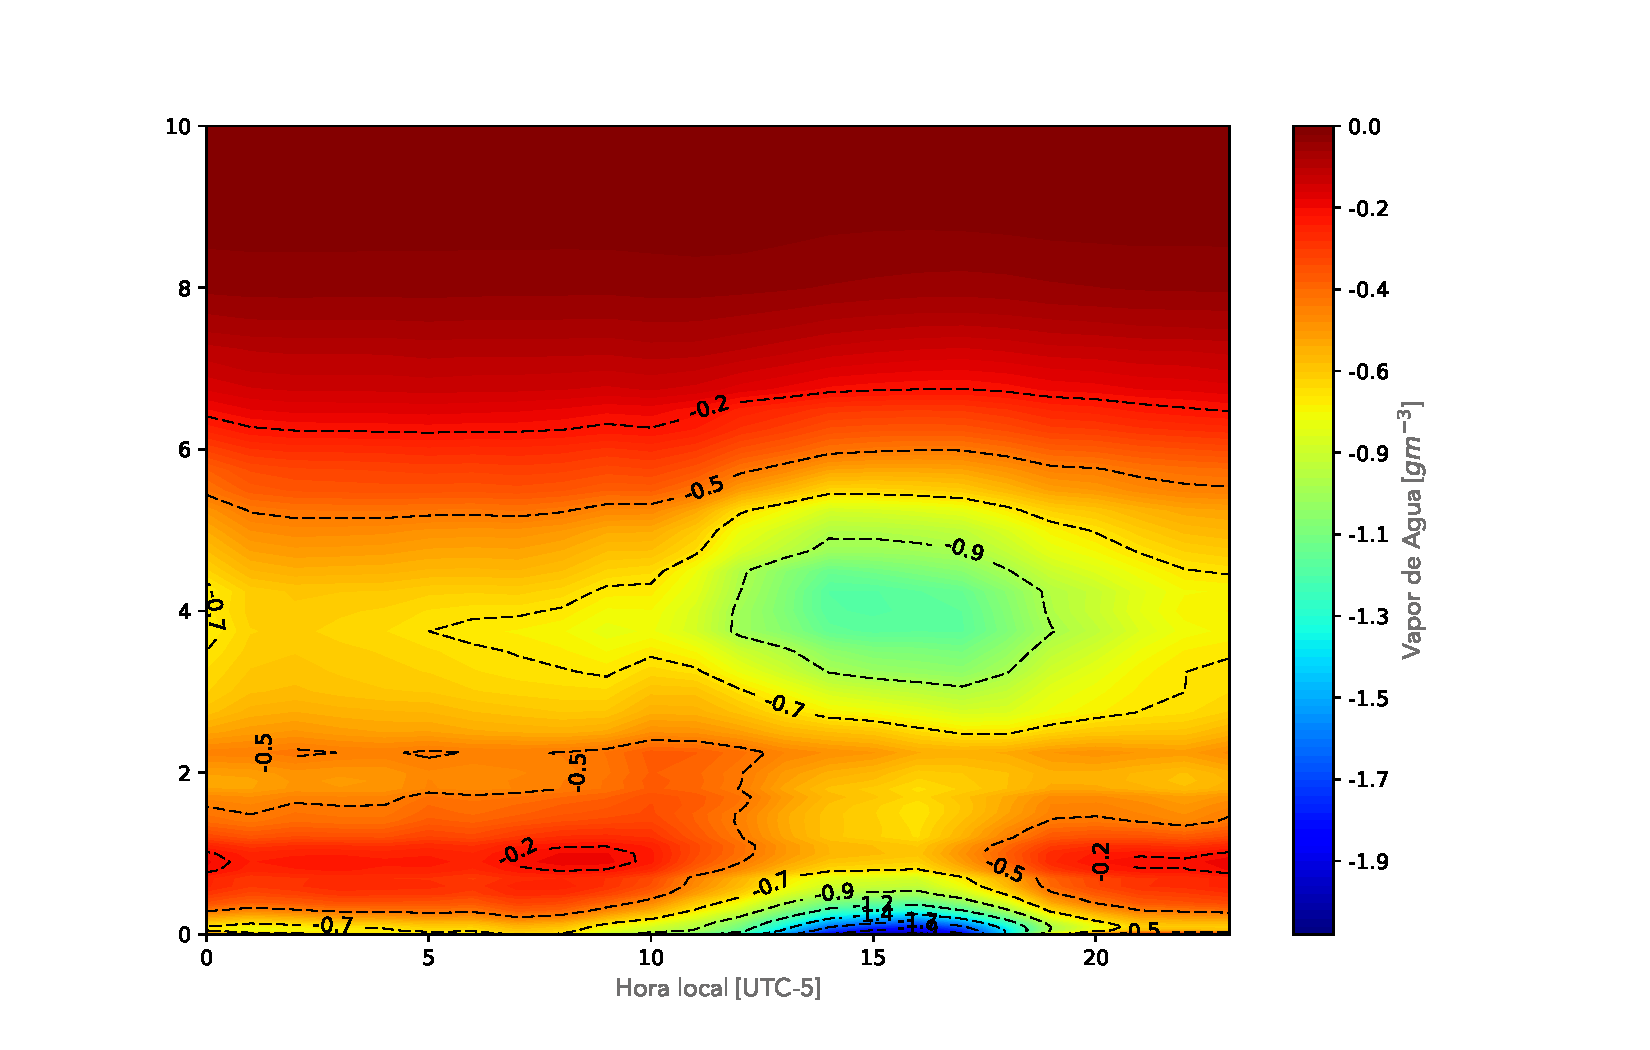
\includegraphics[width=1.2\linewidth]{Figuras/V_C_Matrix_resta.pdf}
\caption{Diurnal cycle difference of water vapor between days with absence or presence of precipitation events }
\label{fig:VaporDifference}
\end{figure}

The diurnal cycle  is not the only either the principal cycle in the variability of the water vapor and precipitation distribution, the annual cycle is another important component of the precipitation an water vapor variability due the radiative forcing, to analyze this cycle the Figure \ref{fig:VapDifference} shows the difference of the annual diurnal cycle of the integrated water vapor column between days with absence of precipitation and the days with presence of precipitation events.

\begin{figure}[h!]
\centering
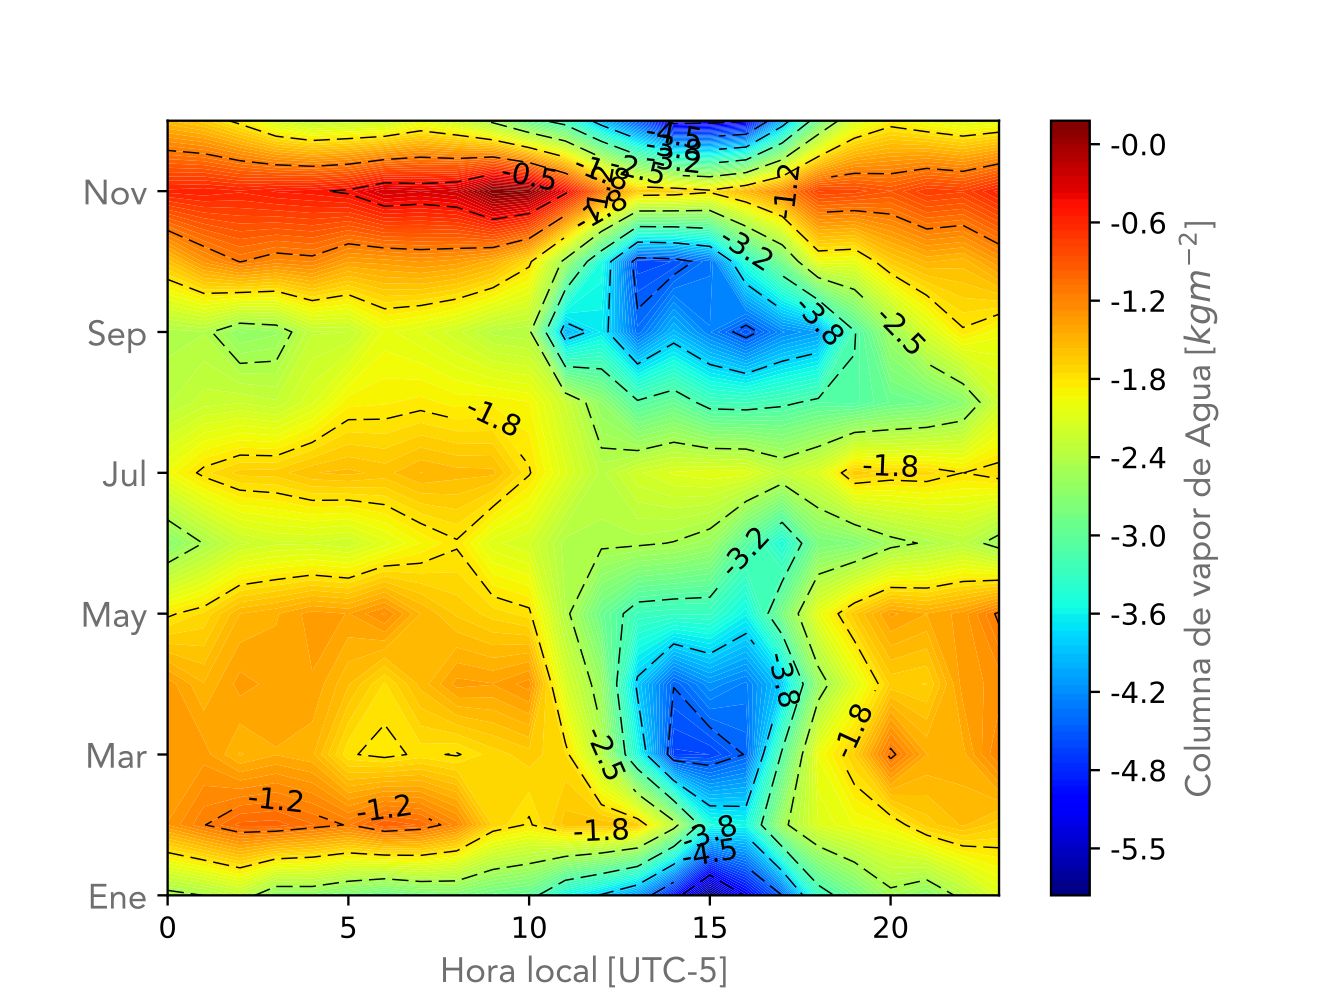
\includegraphics[width=1.0\linewidth]{Figuras/Vap_Resta_Matrix.png}
\caption{Annual diurnal cycle difference of integrated water vapor column between days with absence or presence of precipitation events }
\label{fig:VapDifference}
\end{figure}

The annual cycles modulates the quantity of precipitation and the availability of water vapor due to the passage of the Inter-Tropical Convergence Zone (ITCZ), that demarcates the two rainfall seasons in the colombia's andine zone 



\subsection{Stability indexes}

To analyze the atmospheric stability, i.e. thermodynamic profile, exist indexes that characterizes, with an only value, the state of the thermodynamic profile of the atmosphere. The majority of the indexes were developed empirically with the purpose to measures the atmospheric instability for storm development, besides the indexes are commonly developed and tested in mid latitude zones and flat lands, this increase the importance of evluate the performance of this indexes in tropical zones with mountains and higth altitudes and slopes. (esto es intentando definir topografía compleja). Static stability indexes provide a simple representation of a complex aspect of the atmosphere and are widely used in operational forecasting. However, their applicability is limited, since most are specifically designed to measure deep instability \citep{henry2000static}.

\textbf{Define all indexes in the work, short with references, }

\subsubsection{Showalter index}
This is one of the firts atmospheric stability index, made by \cite{showalter1953stability}. This index evaluete the instability between 850 and 500 hPa, with the buoyant energy at 500 hPa of an air parcel lifted from 850 hPa.


\begin{equation}
SI = T_{500} - T'_{\uparrow_{850}^{500} }
\label{eq:SI}
\end{equation}

where, $T_{500}$ is the ambient temperature at 500 hPa and $T'_{\uparrow_{850}^{500} }$ is the temperature of an parcel adiabaticaly lifted from 850 to 500 hPa.\\

Is important to resalt, the Aburrá Valley bottom are at 1500 meters above mean sea level, near 850 hPa in pressure level, this imply that the parcel ascend are from the surface, different of the soutwestern conditions use by Showalter in his study \citep{peppler1988review}.


\subsubsection{Lifted index}

Is an modification of showalter index made by Galway \cite{galway1956lifted}, and is one of the most use instability index for storm forecasting \cite{peppler1988review}. Similary as the Showalter index, the lifted index evaluate the buoyant energy at 500 hPa of a parcel, but this parcel is adiabaticaly lifted from 50 hPa obove surface. 

\begin{equation}
SI = T_{500} - T'_{\uparrow_{sfc +50}^{500} }
\label{eq:SI}
\end{equation}

where, $T_{500}$ is the ambient temperature at 500 hPa and $T'_{\uparrow_{sfc +50}^{500} }$ is the temperature of an parcel adiabaticaly lifted from 50 hPa above surface to 500 hPa. This is the principal diference with Showalter index in the calculation method.\\


\subsubsection{Convective Aviabable Pontential Energy, CAPE}
The berfore mentioned indexes are function of the instability between two levels in the atmosphere. In adition CAPE is the measurement of the parcel's buoyant energy above the level of free convection (LFC) and below of the level of neutral bouyancy (LNB), is the region where the parcel experiments positive buoyancy after the lifted condensation level (level of parcel's saturation). The amount of CAPE, calulate with the ecuation \ref{eq:CAPE}, represents the integral of buoyant energy between LFC and LNB, the humidity of the profile is consider in the use of virtual temperature. 

\begin{equation}
CAPE = \int_{LFC}^{LNB}g\tfrac{T'_v-T_v}{T_v}dz
\label{eq:CAPE}
\end{equation}

where  $T_v$ is the virtual temperature of the profile, $T'_v$ is the parcel's virtual temperature lifted from the surface, $g$ is the gravity atration, $z$ is the heigth, $LFC$ is the level of free convection and $LNB$ is the level of neutral bouyancy.

\subsubsection{Convective INihibition Energy, CINE}
Is similary calulate as CAPE, but represents the contrary favor to convection. This index repesent the measures of energy in the stability region, i.e. (energy to no favor the lifting berfore LFC) is the region with negative buoyancy before LFC. In the particular case of Aburrá Valley this index is an importan key to understand the development of atmospheric boundary layer and the convection 


\begin{equation}
CINE = \int_{SFC}^{LFC}g\tfrac{T'_v-T_v}{T_v}dz
\label{eq:CINE}
\end{equation}

where $SFC$ is the surface and the other terms are the same of the equation \ref{eq:CAPE}.


\textbf{Include the new graphs and the histograms, thinking to see be better the cycles, include hour precipitation separation}
Put comparision between AIRS, MWR and soundings
\begin{figure}[h!]
\centering
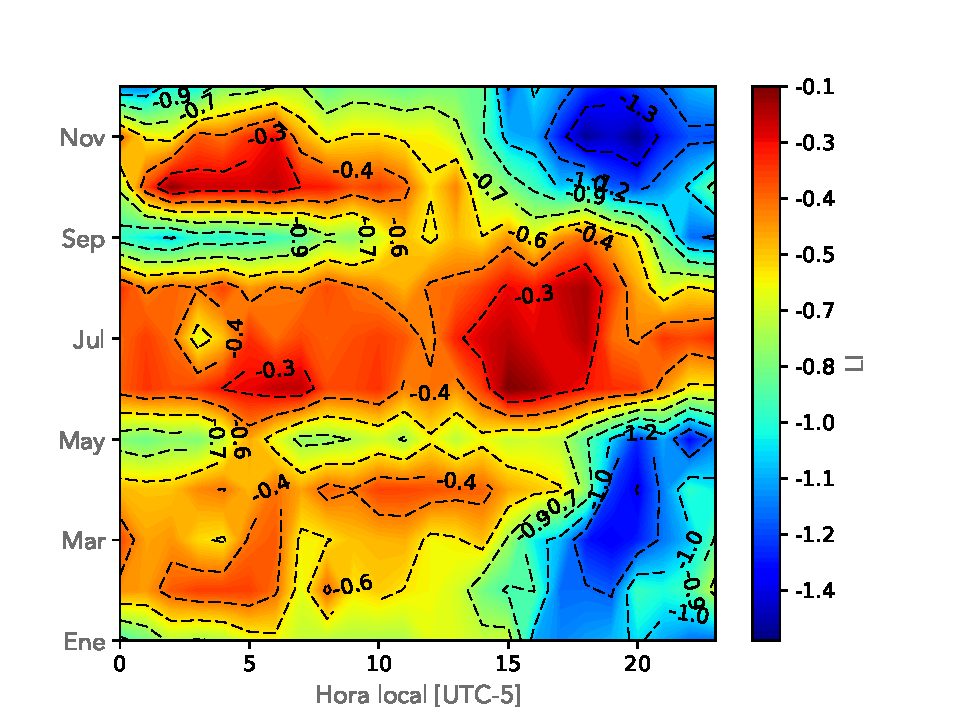
\includegraphics[width=1.0\linewidth]{Figuras/LI_Matrix_resta.pdf}
\caption{Diurnal cycle difference of CAPE between days with absence or presence of precipitation events }
\label{fig:LIdifference}
\end{figure}


\begin{figure}[h!]
\centering
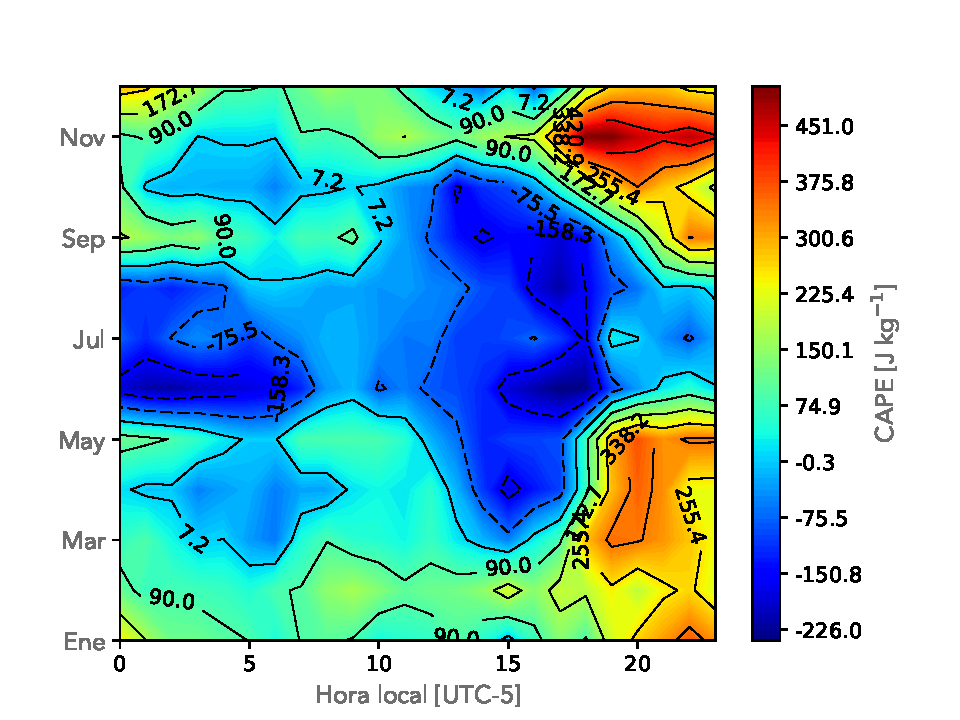
\includegraphics[width=1.0\linewidth]{Figuras/CAPE_Matrix_resta.pdf}
\caption{Diurnal cycle difference of CAPE between days with absence or presence of precipitation events }
\label{fig:CAPEdifference}
\end{figure}

The CAPE Shows the radiative forcing and also important is the more amount of energy available for the days with absence of precipitation, this implicate that the days with precipitation events the potential convective energy is consumed in the precipitation



\begin{figure}[h!]
\centering
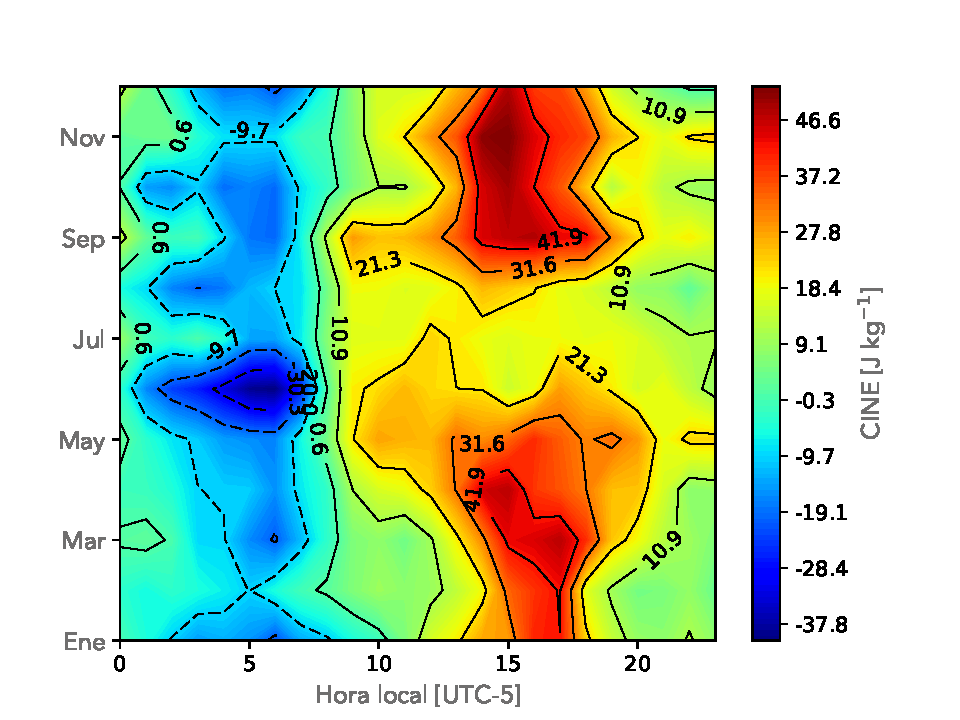
\includegraphics[width=1.0\linewidth]{Figuras/CINE_Matrix_resta.pdf}
\caption{Diurnal cycle difference of CINE between days with absence or presence of precipitation events }
\label{fig:CINEdifference}
\end{figure}


\begin{figure}[h!]
\centering
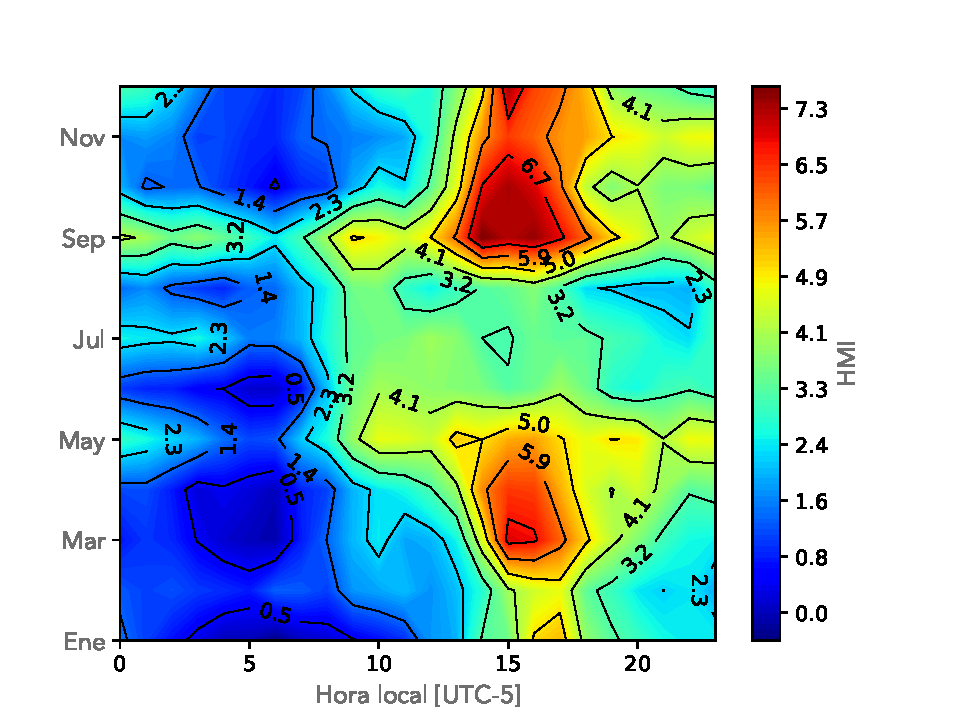
\includegraphics[width=1.0\linewidth]{Figuras/HMI_Matrix_resta.pdf}
\caption{Diurnal cycle difference of HMI between days with absence or presence of precipitation events }
\label{fig:HMIdifference}
\end{figure}

\section*{Data an methodology}
Water vapor sensing methods
\subsection*{AIRS}
Put a graphs an explanation about satellital monitoring, time scale and resolution
\subsection*{Microwave Radiometer}

\subsection*{Soundings}
Comparation with radiometer
\subsection*{WRF}
Comparation

\section*{Results}
Do the plot of histograms o all hours and months

\section*{Conclusions}

%\addcontentsline{toc}{chapter}{\numberline{}References}
%\bibliographystyle{plainnat}
%\bibliographystyle{apalike}
\bibliographystyle{newapa}
\bibliography{Biblio.bib}

\end{document}